\documentclass[11pt]{book}
\usepackage[a4paper, hmargin={4cm, 4cm}]{geometry}
\usepackage{eso-pic} % \AddToShipoutPicture
\usepackage{graphicx} % \includegraphics
\usepackage{minted}
\usepackage{listings}                 % Source code printer for LaTeX
\usepackage{caption}
\usepackage{parcolumns}
\usepackage{fancyhdr}
\usepackage{titlesec}
\usepackage{multirow}
\usepackage{biblatex}
\usepackage{appendix}
\usepackage{tocbibind}

% Here is where you add your own .bib file
\addbibresource{sources.bib}

\pagestyle{fancy}
\fancyhf{}
\fancyhead[RO, LE]{\thepage}
\fancyhead[LO]{\textsl{\leftmark}}
\fancyhead[RE]{\textsl{\rightmark}}

\renewcommand{\sectionmark}[1]{%
\markright{\thesection \ #1}{}}

\renewcommand{\chaptermark}[1]{%
\markboth{\thechapter \ #1}{}}

\titleformat{\chapter}[display]
  {\normalsize \huge  \color{black}}%
  {\flushleft\normalsize %
   \MakeUppercase{\fontfamily{}\fontsize{24}{24}\selectfont\chaptertitlename}\hspace{2ex}%
   {\fontfamily{}\fontsize{40}{40}\selectfont\thechapter}}%
  {10 pt}%
  {\hrule\vspace{10pt}\raggedleft\bfseries\huge}%


%% Change `ku-farve` to `nat-farve` to use SCIENCE's old colors or
%% `natbio-farve` to use SCIENCE's new colors and logo.
\def \ColourPDF {include/natbio-farve}

%% Change `ku-en` to `nat-en` to use the `Faculty of Science` header
\def \TitlePDF   {include/nat-en}  % University of Copenhagen

\title{
  \vspace{3cm}
  \Huge{A WebAssembly Backend for Futhark} \\
  \Large{Msc Thesis}
}

\author{
  \Large{Philip Lassen}
  \\ \texttt{philiplassen@gmail.com} \\
}

\date{
    \today
}



\begin{document}


\AddToShipoutPicture*{\put(0,0){\includegraphics*[viewport=0 0 700 600]{\ColourPDF}}}
\AddToShipoutPicture*{\put(0,602){\includegraphics*[viewport=0 600 700 1600]{\ColourPDF}}}

\AddToShipoutPicture*{\put(0,0){\includegraphics*{\TitlePDF}}}

\clearpage\maketitle
\thispagestyle{empty}
\setcounter{page}{0}
\pagenumbering{roman}
\newpage
\addcontentsline{toc}{chapter}{Abstract}
\begin{center}
    \textbf{Abstract}
\end{center}

Futhark is a high-performance purely functional data-parallel array programming language targeting parallel compute hardware. Futhark has backends for several  compute architectures  and this thesis adds browsers by targeting WebAssembly and threaded WebAssembly. These are browser technologies which map better to the underlying hardware of devices, including multicore CPUs. 

A JavaScript API is developed for easily calling compiled Futhark WebAssembly libraries in the browser. 
The implementation and generated WebAssembly code is benchmarked for both browsers and NodeJS, against the Futhark sequential C and multicore C backends. The sequential WebAssembly performs close to sequential C speeds. The parallel execution of threaded WebAssembly provides a multifactor speedup.


%A large percentage of today's software is run in the browser, and the underlying hardware of the laptops and mobile phones that run these browser have increasingly parallel compute with GPU's and multicore CPU's. As such there is heavy development of standardized cross browser Web API's to harness these parallel architectures. One of these technologies is threaded WebAssembly. This thesis develops WebAssembly and threaded WebAssembly backends for the Futhark programming language, leveraging both parallel computing and browsers as a target architecture.  


\tableofcontents



\chapter{Introduction}

TODO motivation and goals


A large percentage of today's software is run in the browser, and the underlying hardware of the laptops and mobile phones that run these browser have increasingly parallel compute with GPU's and multicore CPU's. As such there is heavy development of standardized cross browser Web API's to harness these parallel architectures. One of these technologies is threaded WebAssembly. %This thesis develops WebAssembly and threaded WebAssembly backends for the Futhark programming language, leveraging both parallel computing and browsers as a target architecture.



\setcounter{page}{1}
\pagenumbering{arabic}
\section{Thesis Structure}


\begin{itemize}
    \item Chapter 2, Background:
    Overview of the related work that this thesis builds on.

    \item Chapter 3, WASM:
    Explanation and analysis of WASM as a programming language and as a target language for the browser. 
    
    \item Chapter 4, WASM  Backend Implementation:
     Description of the implementation of the WASM backend. As well as a overview of the performance bench-marked against the native C backend.
    
    \item Chapter 5, Parallel Compute in the Browser:
    Analysis of the facilities and paradigms for parallel programming in the browser through JavaScript and WASM. 
    
    \item Chapter 6, WASM Multicore Backend Implementation:
    Description of the implementation of the multicore WASM backend. As well as a overview of the performance benchmarked against the native multicore C, and WASM backend developed in Chapter 4.
    
    \item Chapter 7, Conclusion:
    Summary of the implementations and performance of the backends developed. As well as a brief discussion of future developments for Futhark targeting parallel compute in the browser.
    
\end{itemize}
\chapter{Background}

This chapter describes relevant background for the work in this thesis, namely browser programming facilities and the Futhark programming language.






\section{Programming Languages in the Browser}

%\section{Futhark}


%\section{Browsers}

%The first web browsers started as Graphical User Interfaces for rendering static web pages. Web Browsers have evolved to keep up with the high paced innovation in web technologies and with modern day browsers having strong similarities with full blown operating systems. 


%\subsection{JavaScript}

%JavaScript for a long period of time was the only supported programming language for the browser. As such it became one of the largest programming languages in the world. With browsers being one of the most ubiquitous coding platforms, programmers were restricted to JavaScript for any functionality in their websites that run client side. As a result many languages added backends to target JavaScript to that programmers could write code in their respective languages and generate JavaScript that would run in the browser. The problem is that JavaScript is not a particularly good target language, as it was not designed with this use case in mind. 

%http://www.observationalhazard.com/2018/06/history-of-web-programming.html
% ^ This is about the programming languages in the web in the early days vbscript and java applets

In the early days of web browsers, web pages would render differently across browsers as there was no standardization's for web API's. Different browsers supported different programming languages, e.g. Java applets and VBScript, creating big headaches for programmers, who wanted their websites to render identically across browsers. One of the first popular languages for the browser was JavaScript, but the implementations across browsers differed. Eventually the big vendors converged on JavaScript releasing a standardized version called ECMAScript. 

Huge investments have been made to increase the execution speed of JavaScript in the browser. With Google and Mozilla investing heavily into the V8 JavaScript engine and SpyderMonkey, (Add Safari and maybe Opera) respectively. Many approaches have been taken to make JavaScript faster. However they have all been fundamentally limited by the language design. 

%\subsection{ASM.js}

One of the approaches taken by the browser vendors was to define a subset of the language asm.js and a convention for type hints, which were designed for efficient execution by leveraging types and compiler tricks to allow ahead of time compilation. It was intended as a target language for compilation of statically typed programming languages. Emscripten \cite{emcc} was developed to be a C/C++ to asm.js compiler. 

Google also introduces Google Native Client (NaCl)\cite{nacl} as a way to bridge the speed gap between running code in the browser, and natively. NaCl is a sandbox for running compiled C and C++ code in the browser efficiently and securely, independent of the user’s operating system \cite{nacl}. However it struggled to gain adoption due to its lack of portability as it was only supported by Chromium based browsers. 


%\subsection{WASM}
The major browser vendors collaboratively designed WASM \cite{wasm_og} to more comprehensively address the limitations of JavaScript as a target language for the web. It is a portable low level byte code, designed for compact representation, efficient compilation, and near native execution speeds. WASM is gaining adoption and has been used for a variety of applications especially as a target for compilation from C, C++ and Rust. 

Google Earth\cite{google-earth-history} is a computer program, that renders a 3D representation of Earth based primarily on satellite imagery. It started out as a desktop application, but in 2013 was ported to the web. It originally only ran in Chrome, as it was built on NaCl. They tried to build it with asm.js, but found that the binary sizes of compiling over a million lines of code with Emscripten, to be infeasible large. However with the creation of WebAssembly they were able to make a high performance cross browser implementation of Google Earth due to the speed and small binary sizes of WebAssembly \cite{google-earth}.

TensorFlow \cite{tensorflow} is an open source machine learning library, originally written in C++. Due to the large eco-system of JavaScript developers and its ability to run on the browser, they introduced TensorFlow.js \cite{tensorflowjs}. They have multiple backends including a WebAssembly backend due to its high performance traits. An interesting aspect of the TensorFlow.js project is that it provides a libraries for web developers to create machine learning models in their website. 

The portability and execution speed have also led to adoption beyond browsers with use cases ranging from (TODO: DFinity and Edge computing). 

%\section{LLVM}

One of the technologies that has greatly helped the adoption of WASM as a target language is the LLVM \cite{llvm} compiler tool chain. Writing a full compiler from scratch that supports multiple targets is an incredibly time consuming process. In order to have high performance backends for different target architectures such x86 and ARM requires knowledge of many of the low level details of each respective target. An alternative approach is for the Compiler frontend of the source language to take the source code and translate it to the LLVM internal representation. As the LLVM compiler tool-chain can then generate high performance code on all the most common computer architectures. Many of the biggest languages are currently built with or have compiler implementations using LLVM.
LLVM generates WASM and therefore languages that generate LLVM IR have any easy path to WASM code generation. 
Emscripten uses LLVM and can generate WASM in addition to asm.js. It is the most widely used compiler for generating WASM.

\section{Parallel Programming in the Browser}
While WASM has progressed the state of the art of single threaded computation speed in browsers an other avenue for execution speed is parallelism. Browsers have facilities for parallel programming. Javascript supports two different paradigms. Web  workers  and  message  passing  enable  parallel  programming  without  shared  memory. SharedArrayBuffer and atomics enable shared memory multithreading with thread synchronization.  There is a threaded WASM proposal that adds atomic operations to the language, and adds support for SharedArrayBuffers while relying on JavaScript’s web workers to create and join threads. 

TODO mention GPU API's for the browser

\section{Futhark}

Futhark \cite{futhark_phd} is a data parallel programming languages that can generate high performance parallel code for both the CPU and GPU .  Writing GPU code and multicore CPU code is hard. It is both difficult to write the code as there are many low level details required to make competitive and optimal implementations. Futhark is a high level functional programming language, which aims to do the heavy lifting for the user.

Futhark programs are generally written with Second-Order Array Combinators, which are similar to the filter, map, and reduce functions commonly found in many functional programming languages. These functions can be optimized to efficient parallel code. These combinators are surprisingly expressive and be combined to encode code complex programs. To see this in action below is a Futhark implementation of matrix multiply.

\begin{verbatim}
let matmul [n][p][m] (xss: [n][p]t) (yss: [p][m]t): [n][m]t =
    let dotprod v1 v2 = reduce (+) 0 (map2 (*) v1 v2)
    in map (\xs -> map (dotprod xs) (transpose yss)) xss
\end{verbatim}
TODO: EXPLAIN THE CODE!
This serves as an illustration of how a relatively involved operation can be written using SOACs. Not only is the implementation short, it's also fast.

Currently the futhark compiler has C backends generating Cuda, OpenCL, and plain C code. It also two Python backends, one sequential backend, and a PyOpenCL backend. All the backends can be compiled to libraries, making it possible to call Futhark from C or Python applications. 

The plain C code backend comes in two variants, sequential C and multicore C. The latter is a recent addition and generates parallel code using POSIX threads (pthreads) \cite{multicore}. These backends are important for this thesis. Emscripten compiles sequential C to plain WebAssembly, and C with pthreads to threaded WebAssembly. This allows us to bootstrap these two backends to generate efficient code that can run in the browser. 


\chapter{WASM}
This chapter gives an overview of the design and structure of the WebAssembly programming language. This will be driven through an example program, and some performance evaluations and literature review. 



Its important to note that WebAssembly doesn't aim to be a complete replacement for JavaScript. WebAssembly cannot access the DOM for example. WebAssembly was instead designed to have good inter-operation with JavaScript. In practice a developer wanting to get high performance code running in the browser would first write their library in a language such as C or Rust. Then they would compile to WASM, and use JavaScript to call their WebAssembly module in the browser. 




WebAssembly aims to define a portable binary format that can be run in the web with high performance. A WebAssembly file is commonly referred to as a module, and given a \textit{.wasm} file extension. WebAssembly also defines a text format that serves to be a human readable version of the underlying binary format, much in the same way assembly provided a human readable format for machine code. 



\section{WebAssembly Module Structure}

WebAssembly files are segmented into sections. The segmentation of these sections is done so that loading a WASM file is efficient as possible. The sections are structured such that the byte code be compiled in a single pass, and in parallel. Furthermore the code can be parsed and compiled before the complete WASM file has been downloaded, reducing the instantiation time of a WebAssembly module. 

WebAssembly supports 4 number types.
\begin{verbatim}
i32: 32-bit integer
i64: 64-bit integer
f32: 32-bit float
f64: 64-bit float
\end{verbatim}
This has ramifications for inter operation with JavaScript, but is useful with respesct to supporting number types for languages like C/C++ and Rust that aims to be a target language for. 

A WebAssembly function has the following structure.
\begin{verbatim}
( func <signature> <locals> <body> )
\end{verbatim}
The signature gives the function name, parameter types, and return types. The locals are the local variables that will be used in the execution of the function, and the body is the actual implementation of the function. The most used WebAssembly example is the add function. 

\begin{verbatim}
(module
  (func (param $a i32) (param $b i32) (result i32)
    local.get $a
    local.get $b
    i32.add))
\end{verbatim}

The function signature of add specifies the two arguements a and b as i32s and specifies the return type result as i32. There are no locals. The funciton body has three instructions. The instructions \texttt{local.get \$a} and \texttt{local.get \$b} push the two arguments to onto the stack. The instruction \texttt{i32.add} pops the two elements off the stack and pushes their sum. The function returns the number on the stack. 

The body of the function could be replaced with 
\begin{verbatim}
 (i32.add (local.get $a) (local.get $b))
\end{verbatim}
that is, the WebAssembly allows the programmer to use a notation where arguments to instructions are passed as parameters instead of manually being placed on the stack.



%TODO link and ref mdn https://developer.mozilla.org/en-US/docs/WebAssembly/Understanding_the_text_format
\section{Memory}

A notion of memory is needed for writing more complex programs. In a language like C, it is common practice to use pointers to locations in memory, or for writing an array of values. Memory from the perspective of WASM is just an array of bytes that can be read from and written to. WebAssembly has two essential functions for interacting with this array, namely the \textit{load.i32} and \textit{store.i32}, for reading and writing to the array of bytes respectively.

As a motivating example the following C code gives a simple implementation of an place prefix sum.

\begin{verbatim}
void prefix_sum(int* arr, int size) {
  for (i = 1; i < size; i++) {
    arr[i] += arr[i-1];
  }
}
\end{verbatim}
The following code is a WebAssembly implementation of inplace prefix sum.
\begin{verbatim}
  1 (module
  2   (import "env" "memory" (memory $memory 1))
  3   (export "prefixSum" (func $prefixSum))
  4   (func $prefixSum (param $size i32)
  5     (local $offs i32)
  6     (local $acc i32)
  7     (local $last i32)
  8     (local.set $offs (i32.const 4))
  9     (local.set $last (i32.mul (local.get $size) (i32.const 4)))
 10     (local.set $acc (i32.load (i32.const 0)))
 11     loop $forloop
 12       (local.set $acc (i32.add (local.get $acc) 
                         (i32.load (local.get $offs))))
 13       (i32.store (local.get $offs) (local.get $acc))
 14       (local.set $offs (i32.add (local.get $offs) (i32.const 4)))
 15       (br_if $forloop (i32.ne (local.get $offs) 
                                  (local.get $last)))
 16     end $forloop
 17   )
 18 )
\end{verbatim}
% TODO brief description of WASM
% TODO talk about 64k pages

For the implementation a local variable accumulator is set to the first value of the array, and an offset is set to 0. A loop is then entered, where the element at offset in the array is loaded with \texttt{i32.load} added to the accumulator and the result is stored with \texttt{i32.store}. The offset is increased by 4 bytes, and than compared to the local variable last. If it is not equal the loop goes back to the loop on line 12, and repeats.

The most important details of the function implementation for understanding WebAssembly's interaction with memory are the load and store operations, which use byte offsets to address memory. The memory is never explicitly referenced in the function because WebAssembly modules only have one declaration of memory in the memory section, making the array of memory implicit. Memory can either be imported from JavaScript, in which case the memory is created in JavaScript and passed to WebAssembly on instantiation, or alternatively the memory can be exported from WebAssembly, in which case the memory is created in WebAssembly on instantiation and can be accessed in JavaScript afterwards. In line 2 the memory is imported. Where the 
\begin{verbatim}
(import "env" "memory" (memory $memory 1))
\end{verbatim}

the ending 1 sets the size of the memory heap to be 1 page of memory. For WebAssembly 1 page corresponds to 64 kilobytes. Memory is always set to an integral number of pages.


\section{WASM and JavaScript interop}

WebAssembly defines a relatively small set of instructions, which runtimes can translate to native code quickly. However because of this it is unable to complete many of the basic functions of JavaScript. The most clear cut example of this is not having access to the DOM. 
WebAssembly does not have direct access to Web APIs. However it can call imported JavaScript functions. This is the facility that allows it to interact with Web APIs. This simple design feature is incredibly powerful. It is this feature that enables threaded WebAssembly as it can leverage JavaScript's ability to spawn web workers. This will be discussed in greater detail in Chapter 6.

\section{Performance}

The performance of WebAssembly

\section{WASM as a library}

For most practical use cases WebAssembly modules are used as libraries. When compiling C to WASM as a library the Emscripten compiler generates two files. One is a WebAssembly module and the other is JavaScript glue code. This allows web programmers to access all the important elements of WASM from a set of JavaScript functions that the Emscripten runtime defines. This is beneficial for multiple reasons. Firstly working directly with WebAssembly modules is a layer of detail most web developers would like to avoid. Secondly this approach allows a programmer to simply compile their C library and call it from JavaScript. 

\section{WebAssembly in the browser}

With the development of WebAssembly


\section{WASM outside the browser}

There are also a number of applications for WebAssembly outside of the browser. The most standard engine for running WebAssembly outside the browser is Node. Node also uses the V8 engine that is present in Chrome, and other browsers to support WebAssembly. As a result it is a high degree of performance parity with WebAssembly that is run in the browser.

Running Node locally is convenient for rapid prototyping as well as testing. Making tests that run in the browser takes a deal of configuration, and isn't trivial. It is possible to run Chrome, and Firefox as headless browsers for testing purposes, but often it is desirable to test part of WebAssembly functionality


WebAssembly executes within a sand-boxed stack-based environment, which means that running foreign code can only effect the virtual environment that executes the WASM module. This compounded with its competitive performance to native code makes it an ideal candidate for any applications that need to run foreign code. 




\chapter{API Design}

TODO make sure that in previous chapter we explictly explain why WebAssembly is better than JavaScript. 



This chapter describes the implementation of an additional Futhark backend that generates WebAssembly and JavaScript glue code such that Futhark programs can be compiled to libraries that can be run in the browser. The implementation includes an API to invoke the compiled libraries from JavaScript. The implementation is benchmarked in the Chrome browser, and in Node.js and against the C backend.

TODO maybe add some motivation

Firstly we design the JavaScript API. We take inspiration from the Futhark C and Python APIs. Our design factors in the characteristics and limitations of JavScript and WebAssembly. The API is illustrated with an example.



Secondly we implement the backend. We take outset in the existing futhark Sequential C backend and pass the generated C code to the Emscripten compiler for the final compiler pass. The Emscripten generates a WebAssembly module along with JavaScript glue code. We generate additional JavaScript code to wrap our API around the JavaScript code generated by Emscripten.

To illustrate the API and backend implementation working in practice we use the WebAssembly backend to efficiently generate graphics for the mandelbrot set in a webpage.

Finally we benchmark the Futhark backend to quantify its performance. The benchmarks come from the futhark benchmark suite\footnote{https://github.com/diku-dk/futhark-benchmarks}, which are standardized benchmarks to test the performance of Futhark backends against industry standards. The benchmarks show the WebAssembly, both when run in the Browser and run on Node locally, performs between 12\% to 65\% slower than the generated C running locally. 

\section{API Motivation}

In order to make Futhark a practical language for writing libraries that can be called in the browser it is important that it has a simple and efficient API. As discussed in chapter 3 in practice code that is compiled to WebAssembly modules come packaged with a JavaScript file. This file contains the library functions that are exposed to the programmer, where internally these functions handle the interaction with WebAssembly. This allows users of the library to be oblivious of the fact that WebAssembly is being used under the hood, much in the same way that some Python developers are oblivious that numpy is running compiled C under the hood.

A succesful API for calling Futhark in the browser will have the following properties
\begin{enumerate}
    \item It should be convenient, seamlessly integrating with the most commonly used JavaScript number and array data types.
    \item The API should be efficient both with respect to memory usage and runtime speed.
    \item Finally the API should minimize boiler plate code.
\end{enumerate}

\section{Comparing Futhark APIs}

It's insightful to look at the APIs of other languages so that we can copy the elements of the APIs that are effective and avoid the parts that are cumbersome or inefficient. These decisions are constrained by the limitations and capabilities of the target language, which for us is JavaScript and WebAssembly.

An additional reason why it is important to observe the C API is that the WebAssembly backend builds off the sequential C backend. For this reason our design choices for the API are limited to how we can wrap the C API function calls behind JavaScript classes and functions.
%% MAYBE Section not CHAPTER BE MINDFUL YOUNG CHILD

The exposition will be example based. To best illustrate the API designs, we choose an example with multidimensional array inputs and outputs as well as a scalar input. 
\begin{verbatim}
entry scale (scalar : f32) (matrix : [][]f32) = 
  map (map (scalar *)) matrix
\end{verbatim}
This program scale.fut multiplies each element of a matrix by a scalar, and returns the scaled matrix. The implementation isn't important as this code is generated by Futhark. What is important is the way we can pass arguments and capture the return values from this function in the target language. 

TODO: also introduce simple increment example

\subsection{C API}

TODO: do increment example first

When scale.fut is compiled as a C library, the files scale.c and scale.h are generated. The implementation and header files respectively. Listing \ref{lst:c-api} is a C program that interfaces with the generated library. 


\begin{listing}[H] 
        \inputminted[fontsize=\small,baselinestretch=0.5,linenos]{C}{code/compiler/api_examples/example.c}
        \caption{C code for interacting with the C API of the compiled program scale.fut }
                        \label{lst:c-api}    
\end{listing} 

At the top level the API works off of a context and a configuration, futhark\_context, and futhark\_context\_config. The configuration stores choices like debugging. The context manages global information and bookkeeping. Including logging and profiling, and a mutex to guarantee thread safety when used from multiple threads. The API has functions to create these at the beginning and free them at the end. 
\begin{verbatim}
futhark_context_config_new
futhark_context_new
futhark_context_free
futhark_context_config_free
\end{verbatim}

Futhark's primitive types (bool, integers and floats) are represented by corresponding C types.

For arrays futhark generates a C type for every type that appears as an argument or result type in any entry point function in the library. It also generates functions to create, access, and free arrays. For example for the futhark array type [][]f32, the generated header file scale.h declares a type futhark\_f32\_2d and functions futhark\_new\_f32\_2d and futhark\_free\_f32\_2d for creating and freeing arrays of that type. Moreover the API generates functions futhark\_shape\_f32\_2d and futhark\_values\_f32\_2d for getting the shape (dimensions) and values of the futhark array respectively. 

For each entry point function in the library a C function is generated, which takes the futhark context, an output parameter for each type in the result tuple, as well as an input parameter for each argument. The function signature for the generated C function for scale.fut can be seen below.
\begin{verbatim}
int futhark_entry_scale(
  struct futhark_context *ctx,
  struct futhark_f32_2d **out0,
  const float in0, const struct futhark_f32_2d *in1);
\end{verbatim}

Memory management is manual. Both the input array created with futhark\_new\_f32\_2d and the output array returned from futhark\_entry\_scale are freed manually.

\subsection{Python API}

When scale.fut is compiled as a Python libray it generates a single Python file scale.py. It contains a class that can be used to interact with the Python methods.
\begin{listing}[H] 
        \inputminted[fontsize=\small,baselinestretch=0.5,linenos]{C}{code/compiler/api_examples/example.py}
        \caption{64 bit multiplication with 128 bit casting}
        \label{lst:int128}    
\end{listing} 


In order to invoke the python library we import the file. Then we instantiate a scale\_class by calling the scale() method. Finally we invoke the method by calling the entry point function with a scalar input and a 2-dimensional numpy array. All primitive Futhark types conveniently map to primitive numpy types. Numpy ndarrays are made up of these primitive types so passing them in as arguments in the API provides sufficient information. We make sure that the numpy array has values of the correct type by calling the astype function of numpy with 'float32', the numpy equivalent of the futhark primitive 'f32'. The entry point function logically returns a numpy ndarray whose elements have type 'float32'. Interestingly numpy scalars are returned by the Python API if the return time is a scalar. However the entry point function can both accept scalars as normal Python numbers or as numpy scalars.


\subsection{API Comparison}

One of the features of the Python API that make it simpler is that it wraps the context and configuration in a class. For the C backend the context needs to be passed to every function call that interacts with Futhark specific functions. The other big advantage of the Python API is that it utilizes the numpy library which provides convenient classes for representing multidimensional arrays. C does not have a clean representation of multidimensional arrays. This makes the C API more verbose.



\section{JavaScript API}

When designing the JavaScript API we consider both usability and performance. 


%\subsection{Futhark Types to JavaScript Types}
JavaScript has one standard number, which is a 64 bit floating point number. This is typically used to encode all numbers. All the Futhark types u8, u16, u32, i8, i16, i32, f32, f64, and bool except for u64 and i64 can be encoded by a 64 bit float. Fortunately JavaScript recently introduced BigInt in ES2020\footnote{SAY WHAT ES2020} to address this shortcoming of the language. With this there is a way to represent every futhark primitive type with either standard JavaScript numbers, booleans, or BigInts. 

One problem with JavaScript is that it doesn't have a standard package with widespread adoption for scientific computing that gives an efficient encoding of n-dimensional arrays. The standard JavaScript array are more reminiscent of lists and have similar semantics to the list type of Python. A problem is that there is no way to efficiently validate the shape for n-dimensional arrays and the types of its elements. 



%\subsection{TypedArrays}

The approach that many scientific JavaScript libraries take is to accept typed arrays as arguments, as well as arguments for specifying the shape and dimensions of the typed arrays. There are 10 different typed arrays, one for each of the 10 numeric types that Futhark provides. Typed arrays have a number of advantages:

\begin{itemize}
    \item Type Enforcement : typed arrays only store the type that is specified by their constructor. 
    \item Memory Efficiency : typed arrays can store types with less than 64 bit precision more efficiently as they don't need to use 64bit float to also store high order bits. As an example a typed array of 8-bit integers takes an eighth of the space compared to a regular array storing numbers.
    \item Ubiquity : Typed arrays are present in all standard JavaScript runtimes, such as Node.js, and Chrome. They don't need to be imported and are often the return types of scientific libraries such as for image or graphics processing
\end{itemize}


In order to maintain the most flexibility with our API design we choose to both have a way to work with the API through simple JavaScript Arrays, as well as through typed arrays. Typed arrays will have a little extra baggage to carry along shapes.


%\section{JavaScript API}

%\subsection{Types}

Futhark primitive types for all types except i64, u64 and bool are represented by the standard JavaScript number type. i64 and u64 are represented by the BigInt number type. bool is represented by the standard JavaScript boolean type. The type conversion between Futhark types and JavaScript types can be seen in listing \ref{table:types}.

All array values share the same structure API. They can be passed in as n-dimensional arrays of their associated JavaScript type. Note that these arrays must be regular, it is on the caller to enforce this.
Alternatively we provide a FutharkArray class which can be instantiated from typed arrays. FutharkArray instances are also accepted by entry point functions. Users who have a focus on (space and speed) efficiency should elect to use this over regular JavaScript arrays. Users using a more efficient representation of their data with typed arrays aren't forced to convert into a less efficient representation. The type conversion between Futhark types and typed arrays can be seen in listing \ref{table:types}.

Finally there are Opaque types, which don't have a clean mapping from Futhark to JavaScript. Instead they are represented with a FutharkOpaque class. This class doesn't have meaning outside of the context of being passed form the output of one entry point to the input to another entry point with the same type.

\begin{listing}[H] 
\begin{table}[H]
\centering

\begin{tabular}{|c|c|c|}
\hline
\textbf{Futhark Type} & \textbf{JavaScript Type} & \textbf{TypedArray Type} \\ \hline
i8                    & number                   & Int8Array                \\ \hline
i16                   & number                   & Int16Array               \\ \hline
i32                   & number                   & Int32Array               \\ \hline
i64                   & BigInt                   & BigInt64Array            \\ \hline
u8                    & number                   & Uint8Array               \\ \hline
u16                   & number                   & Uint16Array              \\ \hline
u32                   & number                   & Uint32Array              \\ \hline
u64                   & BigInt                   & BigUint64Array           \\ \hline
f32                   & number                   & Float32Array             \\ \hline
f64                   & number                   & Float64array             \\ \hline
bool                  & boolean                  & Uint8Array               \\ \hline
\end{tabular}
\end{table}
\caption{Type conversion table from Futhark types to primitive JavaScript types and TypedArrays.}
\label{table:types}
\end{listing}


\subsection*{FutharkContext}

FutharkContext is a class that contains information about the context and configuration from the C API. It has methods for invoking the Futhark entry points and creating FutharkArrays on the WebAssembly heap. 

It is instantiated with the empty constructor.

\begin{verbatim}
var fc = new FutharkContext();
\end{verbatim}
 
FutharkContext has methods for creating FutharkArrays, one method for each futhark array type that appears as an argument to any entry point function. Each method has the following signature
\begin{verbatim}
    new_<type>_<n>d(typedArray, dim_1, ..., dim_n) 
\end{verbatim}

Working off of the example scale.fut, to create FutharkArray for a matrix of [][]f32, we would make the following call. 

\begin{verbatim}
  var fc = new FutharkContext();
  var typedArray = new Float32Array([0.5, 0.4, 0.3, 0.2, 0.1, 0.0]);
  var futharkArray = fc.new_f32_2d(typedArray, 3, 2);
\end{verbatim}

\subsubsection*{Entry Points}
Each entry point function in the compiled module has a method on the FutharkContext. Scalars parameters are either BigInt numbers, regular JavaScript numbers, or booleans. Array parameters can be either FutharkArrays or, for convenience, JavaScript Arrays.

The method returns an array if the futhark return type is a tuple. Otherwise it returns a single value.

Invoking the entry points of scale.fut looks something like this:

\begin{verbatim}
  var fc = new FutharkContext();
  var typed_array = new Float32Array([0.5, 0.4, 0.3, 0.2, 0.1, 0.0]);
  var fut_arr = fc.new_f32_2d(typed_array, 3, 2);
  var fut_arr_result = fc.scale(0.5, fut_arr);
  console.log(fut_arr_result.toTypedArray(), fut_arr_result.shape());
\end{verbatim}

As stated earlier entry points also allow JavaScript Arrays as inputs, provided they have the correct types and dimensions and are regular. So an alternative approach with JavaScript arrays would look like this:

\begin{verbatim}
  var fc = new FutharkContext();
  var matrix = [[0.5, 0.4], 
                [0.3, 0.2],
                [0.1, 0.0]];
  var fut_arr_result = fc.scale(0.5, matrix);
  console.log(fut_arr_result.toArray());
\end{verbatim}

The second implementation is simpler but also less efficient as regular JavaScript arrays require multiple levels of type conversion under the hood.

The fut\_arr\_result in both the examples is a FutharkArray. FutharkArray has methods for getting the underlying data out into basic JavaScript as either a TypedArray or JavaScript Array.

We omitted calls to free arrays and context in these examples. However this will be discussed in section ? below.

\subsubsection*{FutharkArray}
The FutharkArray allows us to get the underlying data from the WebAssembly Heap to JavaScript. It provides the following methods:

\subsubsection*{toArray()}
Returns a JavaScript array with the correct dimensions.

\subsubsection*{toTypedArray()}
Returns a flat typed array of the underlying data.

\subsubsection*{shape()}
Gives the shape of the FutharkArray as an array of BigInts.

\subsubsection*{futharkType()}
Returns the futhark type of the elements as a string, i.e. "bool", "u32", "i8", etc.

\subsection{Memory Management}

Unfortunately WebAssembly does not have garbage collection. This means that the programmer is responsible for doing this manually. The JavaScript API introduced 3 classes, FutharkContext, FutharkArray, and FutharkOpaque. Each has a free method, which the API user must call manually to free underlying memory on the Emscripten memory heap. 

TODO: point to a code listing that does this.

%This chapter discusses the implementation of the initial WASM backend. It discusses the design choices made with considerations to code maintenance, performance, and practical usability. 

\chapter{Implementation}

\section{WebAssembly Code Generation}

We will now describe the implementation of the WebAssembly backend for Futhark.

The most used WASM backends, namely Rust and C/C++ use LLVM to generate WASM code. The reason they are able to do this successfully is because the languages already have compiler frontends that go from the source language to the LLVM IR. With respect to the Futhark compiler, instead of emitting a standard compiler intermediate representation, it elects to generate C code that can in turn be compiled with any standard C compiler. This has the advantage of portability in the sense that it doesn't depend on LLVM which doesn't come standard on all Windows, and Linux distributions. 
Emscripten provides the facilities for going from C source code to WASM. The alternative to generating LLVM IR for it to produce WASM, is using the Emscripten compiler on the generated C code. The last option is to directly generate WASM from Futhark source code. These three choices will be discussed briefly.

\begin{itemize}
    \item Generating WASM directly: 
        This is the least attractive of all the options. Writing low level code is time consuming and also inefficient, in the sense that it would be nearly impossible to capture enough of the optimizations that modern compilers provide.
    \item LLVM IR: This is the most standard approach among compilers. However since Futhark doesn't already generate LLVM IR utilizing this approach would effectively require a redesign of the compiler architecture. This would be an interesting project, with possible positive implications in more places than just a WASM backend. However this would be quite a large task, as the Futhark frontend wasn't designed with this specific intermediate representation in mind. 
    \item Emscripten: Emscripten can simply take C source code generated from the Futhark compiler. This approach would require the least modifications to the compiler. Futhark also aims to emit high performance C code, and Emscripten aims to translate C to high performance WASM code. Connecting the two compilers together is the approach that is most logical.
\end{itemize}

Conveniently the Emscripten compiler is a full fledged production ready C and C++ to WASM compiler, used by the likes of Google, and Mozilla. In order to test the viability of taking generated C source code and passing it through the Emscripten compiler, some exploratory testing was necessary.

The following minimal program takes a 32 bit integer and returns the successor.
\begin{listing}[H]
\begin{minted}{Haskell}
entry increment (a : i32) = a + 1
\end{minted}
\caption{Futhark implementation of the increment function}
\label{lst:simp}
\end{listing}



However when this code compiles to C. it generates over 2200 lines of code. This is because it contains logic for option parsing, and a fair deal of boiler plate code

TODO say what the boiler plate code is and don't call it boiler plate.


Before going farther with the Emscripten compiler it is a worth while experiment to see what modifications have to be made to the generated C code before it can be accepted by the Emscripten compiler.

One issue was in platform specific code used for timing, however on further inspection it turned out that this code was a relic and not actually used anywhere in the compiler, and therefore could just be deleted.

Listing \ref{lst:int128} gives the other function implementation that Emscripten can't compile.
\begin{listing}[H] 
        \inputminted[fontsize=\small,baselinestretch=0.5,linenos]{C}{code/compiler/int128_c.c}
        \caption{64 bit multiplication with 128 bit casting}
        \label{lst:int128}    
\end{listing} 

The issue is that Emscripten and WASM don't support \textit{uint128} types. Instead an alternatate implementation for calculating the high order bits of 64 bit multiplication that doesn't cast to \textit{uint128} numbers is used. 

\begin{listing}[H] 
        \inputminted[fontsize=\small,baselinestretch=0.5,linenos]{C}{code/compiler/int128_wasm.c}
        \caption{64 bit multiplication without 128 bit casting}
        \label{lst:integrate-js}    
\end{listing} 


With the small modifications described to get the generated C to a state where it can be compiled with the Emscripten compiler, Futhark programs can be compiled to WASM and run with Node as Executables. Note that this is specifically for executables and not C libraries. However it is of most interest to get Futhark running in the browser as a library such that web developers can design high performance libraries in futhark and then call them from JavaScript in their frontend. 


%\subsection{JavaScript and WebAssembly number types}

In order use the JavaScript and WebAssembly code that is generated by Emscripten as a library, the C library functions need to be exported during the Emscripten compilation process. The library functions that need to be exported are the ones that the Futhark C backends emit into the C header file when the futhark program is compiled as a library. Again this whole process works almost out of the box when connecting Futhark's C library code generator with the appropriate Emscripten command. However an issue is that int64 types create cryptic errors when they are provided argument types to functions. 

JavaScript are 64-bit floating-point values. This means that all 32 bit numbers can be represented in JavaScript, but not all 64 bit numbers can be represented with full precision.
%WebAssembly fully support for 64-bit integers. This creates an issue as JavaScript can not call WebAssembly functions with appropriate type. This can be handled by instead passing two arguments to JavaScript functions, one for the low order 32 bits, and another for the high order 32 bits. This method is quite clunky, which is why 
%
Emscripten solves this with BigInts when used with the WASM\_BIGINT compiler flag. This gets 64-bit integers working in C with the caveat that when the function is called from JavaScript, the argument must be provided as a JavaScript BigInt.
% Possibly show function taking two arguements here as an example
%After introducing this compiler flag and with the appropriate functions exported from the header file,  %Reference https://v8.dev/features/wasm-bigint

With these fixes a programmer familiar with the semantics of the Emscripten heap has a workable WASM library.

When Emscripten compiles C code it generates two files. One is a WASM module, which contains the instructions for computing the functions described in the C source code. The other file is JavaScript glue code, which is used to take care of loading the WASM file, as well as handling any JavaScript calls that the WASM module might use.

The WebAssembly module has methods for each function that appears in our .c file, plus some system library functions like malloc and free. To call these functions from JavaScript we must tell Emscripten with the '-s EXPORTED\_FUNCTIONS' compiler flag to export them. The method names are all prefixed with underscore.


Emscripten also offers the getValue function to read a scalar of a specified type stored on the Emscripten heap. For example the function call 'getValue(ptr, 'i32')' reads a 32 bit signed integer from the heap at the memory location given by ptr.






Given all this we can now work with Futhark from JavaScript and do the equivalent of listing \ref{lst:c-api-incr}. Listing \ref{lst:c-api-incr} showed how to call Futhark's generated C library from the increment.fut example. After compiling the C library to WASM with Emscripten, the library can be called with the JavaScript equivalent shown in listing \ref{lst:raw_incr}.

\begin{listing}[H] 
        \inputminted[fontsize=\small,baselinestretch=0.5,linenos]{JavaScript}{code/compiler/api_examples/raw_incr.js}
        \caption{Working with raw Emscripten for the increment function}
        \label{lst:raw_incr}    
\end{listing} 

This is quite cumbersome for a function that simply takes a single integer argument and returns a single integer.
The program is basically a one to one match of the C equivalent from listing \ref{lst:c-api-incr}, including passing around pointers, which is unsafe and not idiomatic in JavaScript.
The allocation and freeing of out\_ptr in lines 5 and 8 are even worse than the equivalent C. They are needed because the output 32-bit integer parameter can only write to the Emscripten heap and therefore the caller must explicitly allocate and free the 4 bytes, and copy out the result with getValue. This isn't the case in C because of the shared address space between the caller and the library function, allowing the caller to pass a pointer to a stack allocated result variable.

The picture gets even worse when the Futhark entry points accept and return array arguments.
These necessitate copying array contents to and from the Emscripten heap, exacerbating the C like manual memory management which is a poor fit in JavaScript. 
To contain this complexity we provide two helper functions: copyToHeap allocates space on the heap and copies bytes from a typed array, and viewHeap returns a typed array which presents a view to underlying bytes on the heap. These functions can be seen in listing \ref{lst:heap-helpers}.
\begin{listing}[H] 
        \inputminted[fontsize=\small,baselinestretch=0.5,linenos]{JavaScript}{code/compiler/api_examples/heap-helpers.js}
        \caption{Heap helper functions}
        \label{lst:heap-helpers}    
\end{listing} 

With these functions we can illustrate how to work with the more complex scale.fut from listing \ref{lst:c-api}. As a reminder the futhark function takes a 2d array of floats and a scalar float as input and returns a 2d array of floats that is element wise scaled by the scalar. 

\begin{listing}[H] 
        \inputminted[fontsize=\small,baselinestretch=0.5,linenos]{JavaScript}{code/compiler/api_examples/raw.js}
        \caption{Working with raw Emscripten }
        \label{lst:raw}    
\end{listing} 

The JavaScript is as tedious as the original C code with respect to manual memory management and, like in the previous example, needs to allocate and free memory on the Emscripten heap to retrieve the out\_ptr output parameter. In this example the output parameter is an array pointer. Pointers default to 32-bit signed integers in WebAssembly.\footnote{TODO: wasm64}

These pain points were motivating reasons for the design of the API. Even with the two helper functions we defined to simplify memory copies and reads, working with the raw functions from Emscripten is only accessible to programmers with a strong understanding of memory in WebAssembly. This isn't reasonable as inter-operation between Futhark and JavaScript is a determining factor in whether Futhark is a good language for writing code to run in the browser. For Futhark to be practical the implementation details of the raw pointers to the heap should hidden by a layer of abstraction. This is precisely what the API designed in Chapter 4 accomplished. 



\begin{listing}[H] 
        \inputminted[fontsize=\small,baselinestretch=0.5,linenos]{JavaScript}{code/compiler/api_examples/FutharkContext_incr.js}
        \caption{FutharkContext class for the futhark increment function}
        \label{lst:FutharkContext_incr}    
\end{listing} 







\begin{listing}[H] 
        \inputminted[fontsize=\small,baselinestretch=0.5,linenos]{JavaScript}{code/compiler/api_examples/FutharkArray.js}
        \caption{Class FutharkArray}
        \label{lst:FutharkArray}    
\end{listing} 

TODO explain FutharkContext

\begin{listing}[H] 
        \inputminted[fontsize=\small,baselinestretch=0.5,linenos]{JavaScript}{code/compiler/api_examples/FutharkContext.js}
        \caption{Class FutharkContext}
        \label{lst:FutharkContext}    
\end{listing} 

TODO opaque types


\section{Compiler Pipeline}

When putting all these pieces together and adding the modifications in the compiler an important implementation observation is that the API only depends on 3 things. The name of Futhark's C library functions, these functions' return types, and these functions' arguments types. This greatly simplifies the implementation. The function names, return types, and argument types are needed for generating the runtime classes, and exporting the functions to the emcc command. Firstly Futhark's C API is a part of the compiler that is most stable. Only depending on this part of the futhark compiler to generate JavaScript code means this section will rarely have to be adapted to deal with code changes in the intermediate representation of the compiler.

%When Emscripten compiles C code it generates two files. One is a WASM module, which contains the instructions for computing the functions described in the C source code. The other file is JavaScript glue code, which is used to take care of loading the WASM file, as well as handling any JavaScript calls that the WASM module might use. In order to have a WASM module that could be easily used as a library without exposing the low level details of C, the FutharkValue and FutharkContext classes were introduced. 

Emscripten provides facilities for combining the JavaScript glue code with a library at a command line with the --post-fix and --js-library flags. This is convenient as it reduces the number of files that are produced from running the \textit{futhark wasm} command.



Figure \ref{fig:wasm} illustrates the logical flow of the compilation of the WASM backend. 

\begin{figure}[htbp]
\centerline{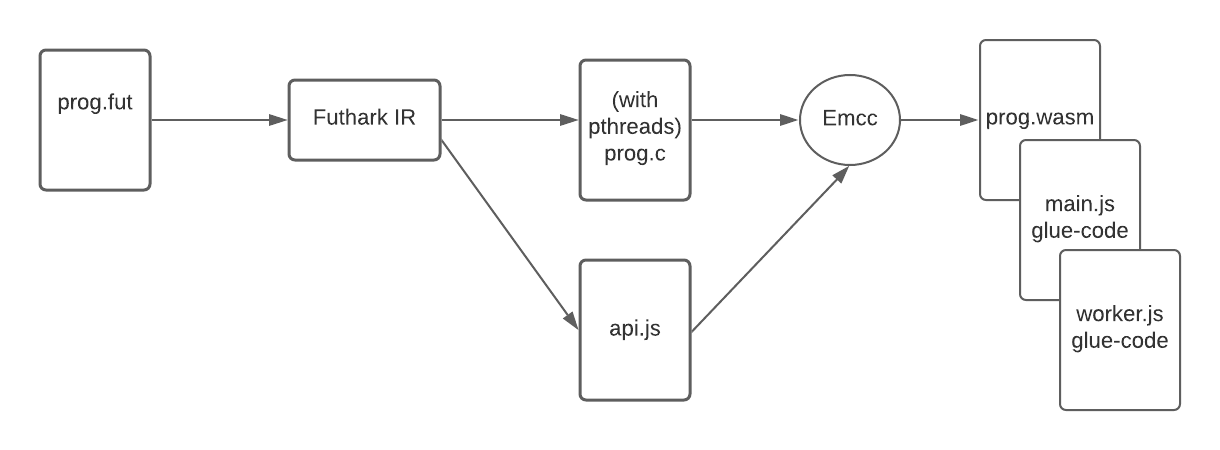
\includegraphics[width=\textwidth]{figures/WASM_MC_compiler.png}}
\caption{WASM-multicore compilation}
\label{fig:wasm}
\end{figure}

The source program is turned into Futhark's intermediate representation, and than into C source code from there. Where as the runtime classes that the WASM backend generates only depend only depend on a the function names, argument types, and return types, which can easily be taken from the IR. At this stage both the C source code and the API are joined together with the EMCC command, generating glue code with the attached runtime code, and a WASM module. 

\subsection{Emscripten Compiler Flags}
The Emscripten compiler provides a large number of flags that effect the usage and the performance of the generated WASM code. Some of the flags are specific to the use case, in which case it makes sense to give the programmer flexibiliy in terms of what compiler flags they elect to use. For this reason the flags the backend implementation elects to only use few flags. As discussed previously in order for 64-bit integers to be handled correctly, the backend needs to use the WASM\_BIGINT flag. The other flag that it defaults to is the O3 optimization level. Though this obfuscates the resulting code, it comes with sizeable performance improvements over the other optimization levels.

The most important flag for users of the WASM backend is the memory flag. The memory flag in Emscripten defaults to 16 megabytes, but with performance heavy computation it is likely that this limit will be exceeded. In these cases the user should manually set the memory based on their needs. It is recommended to use less than 2 gigabytes as only recently have virtual machines started to allow more than 2 gigabytes of heap space. This means that using more memory than 2gb's will likely not be portable across browsers and with different WASM engines. 

\begin{listing}
\begin{minted}{bash}
EMCFLAGS="-s MEMORY=((16777216 * 4))" futhark wasm --lib prog.fut
\end{minted}
\caption{Example futhark wasm compile command}
\label{lst:fu-wasm-compile}
\end{listing}

Listing \ref{lst:fu-wasm-compile} shows an example of calling the backend with an additional compiler flag to set the memory limit higher. The additional compiler flags to Emscripten are passed through the environment variable EMCFLAGS. In this case the memory is increased to 64 megabytes.
\section{Application}

With the WASM backend implemented as described above, it can now be seen in action. One of the applications for high performance computing in the browser is graphics. Figure \ref{fig:mandelbrot} illustrates a Futhark program running in the browser for visualizing the mandelbrot set. First mandelbrot.fut file is compiled as a lib. Than a web server is launched. When the HTML in (TODO cite appendix) is run the webpage in figure \ref{fig:mandelbrot} is rendered.



\begin{figure}[htbp]
    \centering
    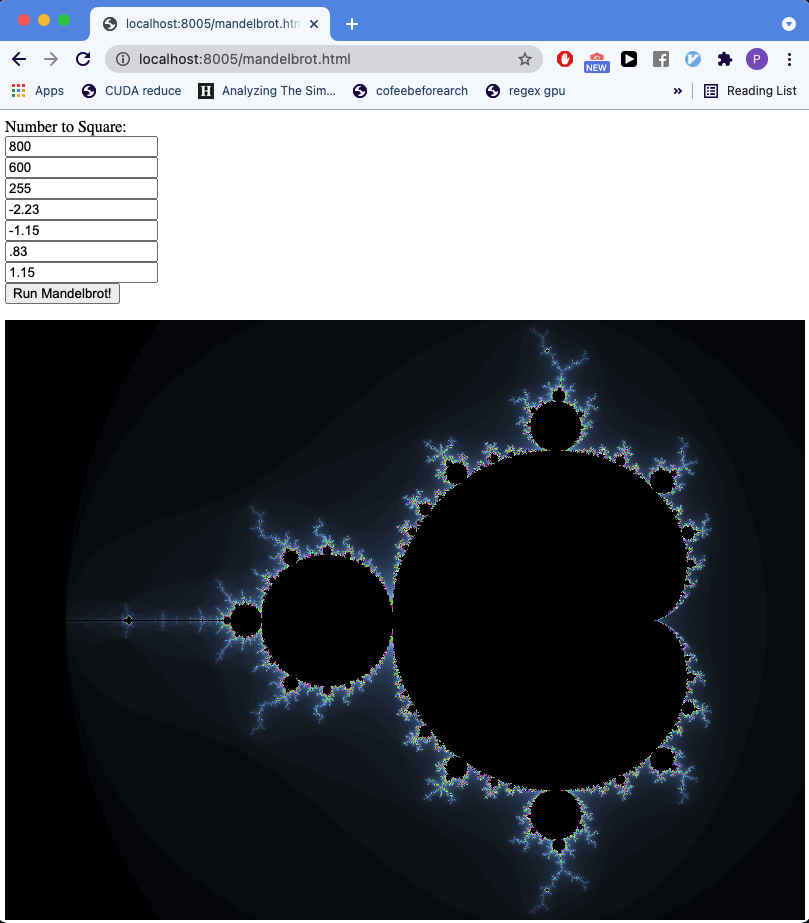
\includegraphics[scale=0.3]{figures/mandelbrot.png}
    \caption{Caption}
    \label{fig:mandelbrot}
\end{figure}

The only Futhark specific code required in to get the values to render is given below. The code is easy to call, and clearly hides the underlying pointers that are being passed around from the programmer.

\begin{minted}{javascript}
var fc = new FutharkContext();
var result = fc.main(screenX, screenY, depth, xmin, ymin, xmax, ymax);
var vals = result[0].values();
\end{minted}

\section{Benchmarking}

The WASM backend is benchmarked against the C backend to see how competitive the execution speed is. The WASM backend is both benchmarked running in the browser with Chrome as well as running with Node. 
\begin{itemize}
    \item Chrome: benchmarking WASM in Chrome gives details on how WASM performs in the browser, which is likely where the backend will be deployed in practice.
    \item Node: benchmarking with Node gives details into how the WASM preforms when run as a backend language. This is interesting as it gives details into the WASM's performance for use cases outside of the browser.
\end{itemize}



The Futhark programs that are benchmarked come from the Futhark benchmark suite, which are used for standardized benchmarks to test the performance of all Futhark backends against industry standards. What is interesting to look at is how the WASM performs relative to the C backend it is built on top of.
\begin{table}[h!]
    \noindent\makebox[\textwidth]{%
    \begin{tabular}{|l|l|l|l|l|l|}
    \hline
    Suite      & Dataset                     & Size & C        & WASM     & chrome \\ \hline
    \multirow{3}{*}{Accelerate} & \multirow{3}{*}{Tunnel} & 1000 & 735 ms  & 1,219 ms  & 1217  \\ \cline{3-6} 
               &                             & 2000 & 2,942 ms & 4,889 ms & 4,827 ms    \\ \cline{3-6} 
               &                             & 4000 & 11,762 ms & 19,693 ms & 19,302 ms   \\ \hline
    \end{tabular}%
    }
    \caption{Caption}
    \label{tab:my_label}
\end{table}

The Tunnel Benchmark shows that the WASM backend takes approximately 65\% performance penalty for running the benchmarks with WASM relative to the sequential C backend. This performance penalty is consistent as the dataset increases, which means that it is not a constant overhead of launching or instantiating WASM. WASM when run in Chrome and in Node have nearly identical performance, with the difference never exceeding 2 percentage points.

\begin{table}[h!]
    \noindent\makebox[\textwidth]{%
    \begin{tabular}{|l|l|l|l|l|l|}
    \hline
    Suite      & Dataset                     & Size & C        & WASM     & chrome \\ \hline
    \multirow{3}{*}{Accelerate} & \multirow{3}{*}{Mandelbrot} & 1000 & 131 ms   & 149 ms  & TODO ms  \\ \cline{3-6} 
               &                             & 2000 & 530 ms  & 602 ms  & TODO ms    \\ \cline{3-6} 
               &                             & 4000 & 2,117 ms & 2,403 ms & TODO ms   \\ \hline
    \end{tabular}%
    }
    \caption{Caption}
    \label{tab:my_label}
\end{table}

For the mandelbrot benchmarks the WASM backend has more competitive execution speeds. The WASM backend is consistently 13-14\% slower across all the sizes. Similarly to the tunnel backend the relative performance difference of the C backend and the WASM does not change with respect to the dataset sizes.


TODO add more benchmarks

TODO add more discussion

TOOO add conclusion
\chapter{Parallel Execution in the Browser}


Browsers have facilities for parallel programming. Javascript supports two different paradigms. Web workers and message passing enable parallel programming without shared memory. SharedArrayBuffer and atomics enable shared memory multithreading with thread synchronization. There is a threaded WASM proposal that adds atomic operations to the language, and adds support for SharedArrayBuffers while relying on JavaScript's web workers to create and join threads. This chapter introduces all these concepts and illustrates them with examples.

JavaScript is single threaded. Meaning it consists of a single call stack and a single memory heap. This is slightly counter intuitive as idiomatic JavaScript often contains many asynchronous function calls. Asynchronous function calls are achieved by placing promises/callbacks into an event queue, which runs after the main thread has finished processing. This way they avoid blocking synchronous JavaScript code from running. 

%There are three primitives used for doing multithreaded programming in the browser: Web Workers, Shared Memory, and Atomics. These features will be introduced in this section along with examples illustrating how they are used in practice. 


\section{Web Workers}
Parallelism with JavaScript in browsers is achieved through web workers. Web workers are extra threads of execution beyond the main thread. The threads interact via message passing. Typically messages are passed through the postMessage and onmessage. postMessage is used to send a message between threads and onmessage works as an event handler to receive messages from threads. 


Web workers are relatively heavyweight, and should not be created in large numbers. They are expected to be long lived and have both high start and high per instance memory cost. 
TODO show why/where this information comes from (FOLLOW UP FROM ABOVE)

The following example computes the Riemann integral of sine over an interval from 0. The interval is broken up into subintervals which are computed by separate workers.

\begin{listing}[H] 
        \inputminted[fontsize=\small,baselinestretch=0.5,linenos]{javascript}{code/worker/integrate.js}
        \caption{Main file that calls workers which handle the computation of Riemann integral} 
        
        \label{lst:integrate-js}    
\end{listing} 

The example code in Listing \ref{lst:integrate-js} spawns 4 worker threads in lines 5-7. It sends each thread a message with their respective index in lines 18-20. It asynchronously waits for messages from each of the worker threads with their partial result and prints the final result when all the threads have sent a message in lines 10-16.
\begin{listing}[H] 
        \inputminted[fontsize=\small,baselinestretch=0.5,linenos]{javascript}{code/worker/worker.js}
        \caption{Worker thread logic for computing Riemann integral} 
        \label{lst:worker-js}    
\end{listing}    

The code in Listing \ref{lst:worker-js} contains the implementation of the worker threads. Once the thread receives a message from the main thread with their index, they compute the partial Riemann integral over their respective quartile of the interval adding the value of sine(x) as many times as specified by granularity. Figure \ref{png:integrate} shows the execution time of the code against a different number of web workers.



\begin{figure}[H]
\centerline{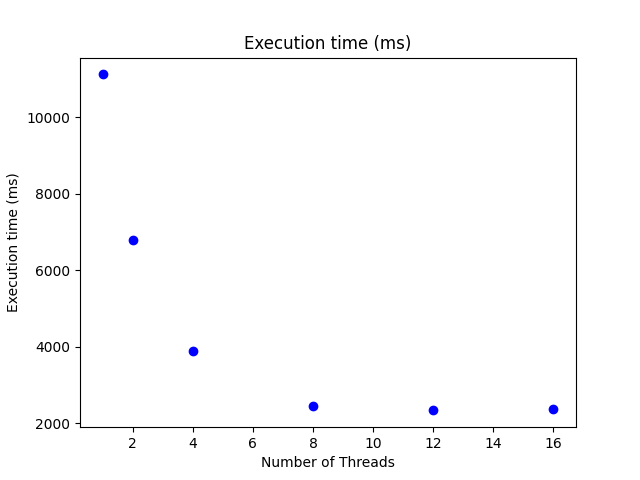
\includegraphics[width=\textwidth]{figures/integrate_exe_times.png}}
\caption{Execution time of Riemann integration for different thread counts. Run on a Macbook Pro with 2,2 GHz 6-Core Intel Core i7}
\label{png:integrate}
\end{figure}

The code execution time in \ref{png:integrate} is for the Reimann integral computed with one billion sample values. For one worker thread the execution time was 11.11 seconds. For two threads the execution time was 6.8 seconds, which is nearly double as fast. However as the number of threads increases the increase in execution speed tapers off. Going from 8 to 12 cores only yields a marginal increase in execution speed going from 2.45 second to 2.39. Once more than twelve worker threads are exceeded, there is no longer a marginal increase in speedup. This can be attributed to the physical limitation of threads on the hardware the code was executed on. The number of logical cores on the computer that executed this code was 12, meaning that any additional web worker launched after the initial 12 must wait on the thread pool for another to finish before it can be activated. In which case the overhead of launching it is only detrimental to the complete execution time of the program


\section{Shared Memory and Atomics}

Web workers with message passing have some similarities in how parallelism is executed with the Erlang programming language. Both of which use message passing to coordinate parallel execution. However many other programming languages and libraries also support and utilize shared memory. An example of this is C/C++ and POSIX threads. Shared memory maps closely to modern multicore hardware, and is faster for certain workloads (TODO GIVE EXAMPLE). However it comes at the cost of a new set of bugs in the shape of data races, which is why languages such as Erlang and Futhark itself abstracts the construct away from the programmer.

JavaScript also offers shared memory through SharedArrayBuffers. A SharedArrayBuffer points to a piece of linear memory. The SharedArrayBuffer can be passed to multiple web workers who can access the memory in parallel. 

In principle safe access to shared memory can be coordinated with message passing, but it's far more efficient for fine grained synchronization to use atomic operations, which again map efficiently to the underlying hardware. Atomic operations make sure that predictable values are written and read, that operations are finished before the next operation starts and that operations are not interrupted (TODO cite Atomics Javascript page). The Atomics package in JavaScript contains functions for performing atomic operations on SharedArrayBuffers. The Atomics package also includes wait and notify functions, like linux futex wait and wake.

To illustrate shared memory and atomics the following example is an implementation of prefix sum. It is a fundamental parallel algorithm which is used as a building block for many other parallel algorithms. The example implements the shared memory 2 pass algorithm from (TODO). 
\begin{listing}[H]    
        \inputminted[fontsize=\small,baselinestretch=0.5,linenos]{javascript}{code/shared/main.js}
        \caption{Main file that calls workers which compute prefix sum using shared memory and atomics in parallel}    
        \label{lst:main-js}    
\end{listing}    
The code in Listing \ref{lst:main-js} spawns 9 worker threads. It sends a message to each of the threads with parameters, some of which are shared array buffers. This allows each of the threads to have access to shared memory. When each thread has sent a message to indicate completion, the final result of prefix sum is logged to the console.

%\captionof{listing}{Example of a worker working}
\begin{listing}[H]    
\inputminted[fontsize=\small,baselinestretch=0.5,linenos]{javascript}{code/shared/prefix_sum.js}
        \caption{Worker file for computing the prefix sum using shared memory and atomics.}    
        \label{lst:prefixsum-js}    
\end{listing}    


The code in Listing \ref{lst:prefixsum-js} handles the actual execution of prefix sum. In the first pass of the algorithm, each thread calculates the prefix sum of their partition in the array, by calling the function prefix\_sum\_partition. Each thread signals that they are done with their work in the first pass by using the Atomics add, and notify functions. The first thread detects signal has accumulated a response of num\_workers - 1, by using the Atomics function wait. At this point the the first thread calculates the cumulative sums of partitions. At this stage it notifies the other other threads using the Atomics store and notify. At this stage all threads calculate the final prefix\_sum, using the precomputed values. On completion each thread sends a message back to the the main file using the postMessage to indicate they are done. 


%TODO: Show speed up over one worker vs 9 workers

%TODO update code to be cleaner and easier to explain

\section{Threaded WebAssembly}
There is a proposal to extend the WASM specification with support for threads, namely by leveraging web workers, shared memory, and atomics. Chrome and Firefox and Node.js all have experimental support for threaded WASM. Emscripten supports compilation of C/C++ with pthreads to threaded WASM.

Threaded WASM uses web workers to create and join threads. It doesn't natively invoke web workers but instead handles this by calling out to JavaScript. Shared memory is accomplished by integrating SharedArrayBuffer with WASM's paged memory model. WASM is extended with atomic operation instructions. Putting it concisely the additions of supporting shared array buffers in WASM and adding atomic operations in WASM was all that was needed to facilitate threaded WASM.

A key observation is that WASM does not natively allow for spawning of threads. This is actually taken care of by the runtime or compiler. Specifically for Emscripten, compiling C code written with pthreads will generate three files. It will generate a WASM file, and and two Javascript files. One for the main glue code and other for worker glue code. The glue code takes care of loading the WASM module, populating the memory with the required values, and integrating with the host system as the C code would expect. The C function pthread\_create is translated to Javascript and not WASM. It launches a Javascript Worker, passing it a shared array buffer and the wasm module that it should run. The WASM simply needs the shared array buffer and atomics to synchronize.  

\begin{figure}[htb]
\centerline{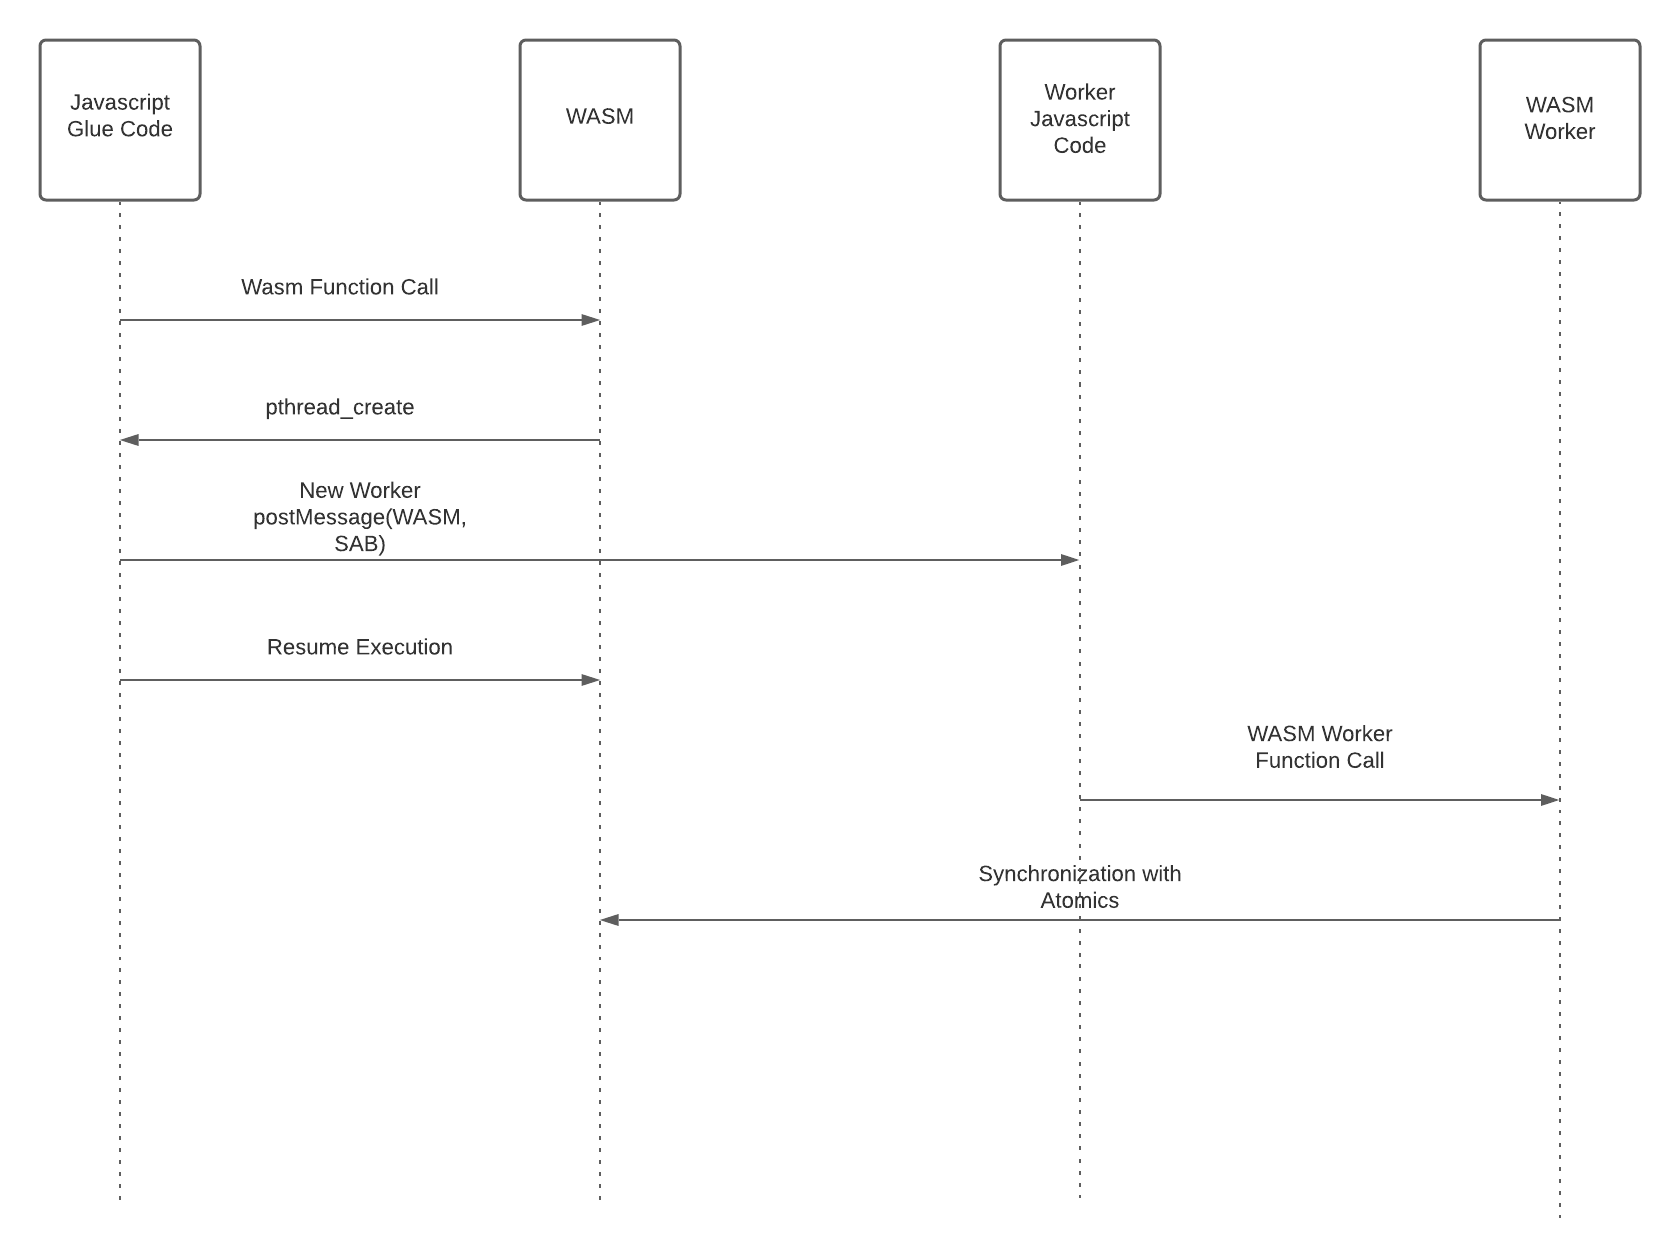
\includegraphics[width=\textwidth]{figures/UML_threaded_wasm.png}}
\caption{UML diagram showing flow of execution of threaded programs in WASM}
\label{uml}
\end{figure}

%TODO make updates to UML as specified on piece of paper.

The UML diagram in figure \ref{uml} demonstrates the execution flow of a parallel function written with pthreads in C, compiled by Emscripten, and run in Javascript and WASM. The javascript glue code calls the parallel WASM function, which then calls an external Javascript function that is used to emulate the functionality of pthread\_create. This function launches a new worker, sending it a message with the WASM module, and a shared array buffer, and resumes execution. This JavaScript worker code then  instantiates the WASM module, calling the designated WASM module function. And then with these multiple WASM modules running in parallel, they use atomic instructions native to WASM to facilitate synchronization, as specified in the program.

%TODO: Pthreads + memory growth talk about this

%TODO: Talk about specifying number of web workers up front with Emscripten

%TODO Explain why threaded WASM has no drawbacks becuase it uses the same facilites as javascript for parralel programming while having the speed up of WASM over JS. (Possibly look at over head of launching/loading WASM in a JS worker file).

\newpage
\chapter{WASM Multicore Backend}

This chapter details the extensions that are added to the Futhark compiler to support a multicore WASM backend. It also benchmarks the generated WASM-multicore code against the sequential WASM backend. It also compares the multicore C backend against the WASM-multicore backend running in the browser.

Fortunately only small adaptions had to be made to the WASM backend developed earlier, to get it running with Multicore. The Futhark compiler has a backend that generates both Sequential C code as well as a backend that generates multicore C code using POSIX threads. As discussed Emscripten can translate multicore C code that uses POSIX threads to multicore WASM that can run in parallel in the browser. The JavaScript API developed in chapter 4 stays unchanged for the WASM-multicore backend. 

Though this thesis adds 2 backends to the 6 backends already present in the Futhark compiler (4 C backends, and 2 Python backends), the added complexity is relatively modest because of the high degree of reuse of code between the two WASM backends. 


\section{Implementation Structure}

Below we discuss how to add a new futhark backend that can be invoked from the command line with \texttt{futhark wasm-multicore}. It is structured very similarly to the plain WebAssembly backend described chapter 4. Instead of calling Emscripten on the Sequential C, we apply it to Futhark's multicore C backend. We utilize the JavaScript and WebAssembly runtime code written in chapter 4, for the backend and add the necessary Emscripten compiler flags required to enable Multicore WASM. Figure \ref{fig:wasm-mc} illustrates the structure of the WASM multicore implementation.

\begin{figure}[htbp]
\centerline{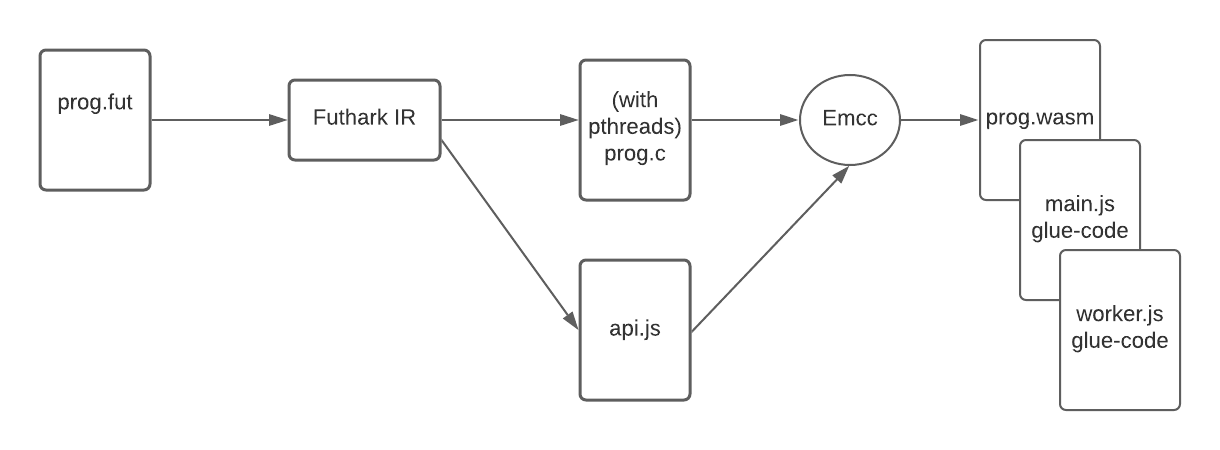
\includegraphics[width=\textwidth]{figures/WASM_MC_compiler.png}}
    \caption{WASM-multicore compilation}
\label{fig:wasm-mc}
\end{figure}
One of the key differences that can be seen in the figure \ref{fig:wasm-mc} is that the wasm-multicore backend produces 2 JavaScript files and 1 WASM file as opposed to the Sequential Wasm backend which generates 1 JavaScript file and 1 WASM file. The second JavaScript file is the web worker glue code.

\section{Implementation Details}
Here we discuss the series of steps that were needed complete the implementation.
\subsection{Plumbing}

We simply combine the multicore C compiler with the JavaScript code generation discussed in chapter 4, by calling the respective functions that contain the meat of the logic, which have already been developed. The last thing of note is that the flag \textit{-pthread} is passed to \textit{runEMCC}. This flag lets Emcc know that our C code contains pthreads, and thereby compiles it correctly.


\subsection{Multicore C code changes}
The pthread C code generated by the multicore C backend used platform specific implementations in the generated function \textit{getrusage\_thread} and \textit{num\_processors}. For \textit{getrusage\_thread} it was possible to reuse the linux implementation. For \textit{num\_processors} it was necessary to add an additional implementation for the Emscripten platform. This was simply done by including \textit{emscripten/threading.h} and calling the function \textit{emscripten\_num\_logical\_cores}.




\subsection{Emscripten Invocation}

The generated multicore C code uses the POSIX function \textit{pthread\_create}. Emscripten aims to follow the POSIX standard closely, but in some places has slightly different behaviour. This is the case for \textit{pthread\_create}, which is a function that is used in the generated multicore C code. 

When pthread\_create() is called, if we need to create a new Web Worker, then that requires returning the main event loop. That is, you cannot call pthread\_create and then keep running code synchronously that expects the worker to start running - it will only run after you return to the event loop (TODO cite pthread docs). In order to work around the API differences, the compiler flag \textit{PTHREAD\_POOL\_SIZE=<integer>} needs to be passed to the Emscripten compiler. This effectively creates the web workers before the main thread is called, in which case create\_pthread can just use an already spawned web worker. From testing, this parameter is best set to the number of logical\_cores of the underlying hardware.





\subsection{Running in browser with HTTP}




\begin{figure}[htbp]
    \centering
    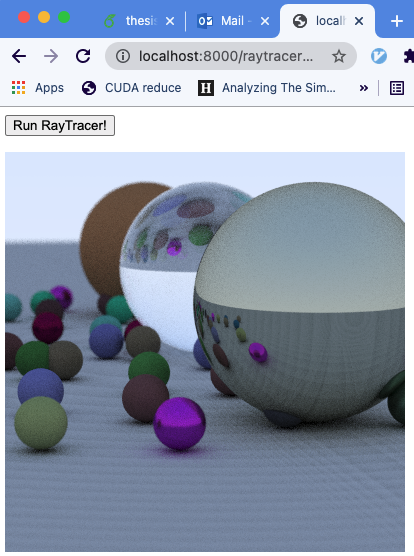
\includegraphics[scale=0.6]{figures/raytracer.png}
    \caption{Caption}
    \label{fig:mandelbrot}
\end{figure}

\section{Benchmark}
\chapter{Conclusion}

TODO


\appendix
\chapter{Source Code}

TODO



\printbibliography[heading=bibintoc]

\end{document}
